\nxsection{Les Comptes Utilisateurs}
\index{les comptes utilisateurs}

\nxsubsection{Afficher les d\'etails d'un compte utilisateur}
\index{afficher les d\'etails d'un compte utilisateur}
\index{d\'etails d'un compte utilisateur}

\begin{figure}[!htpb]
	\centering
	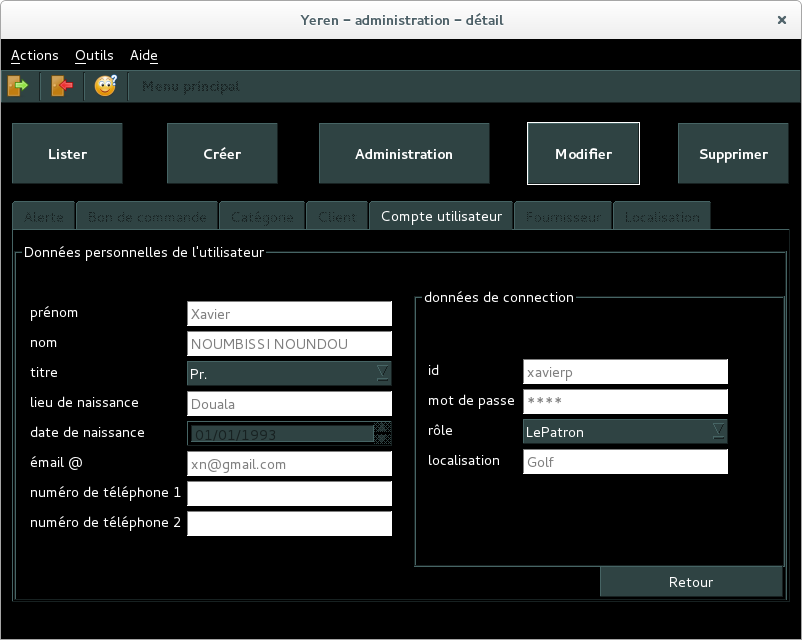
\includegraphics[scale=0.45]{images/compte-utilisateur-afficher-details.png}
	\caption{L'interface graphique pour afficher les d\'etails
			d'un compte utilisateur.}
	\label{fig:admin-comptes-utilisateurs-afficher-details}
\end{figure}

La figure~\ref{fig:admin-comptes-utilisateurs-afficher-details}
illustre l'interface graphique de \yeren qui affiche les
d\'etails d'un compte utilisateur.

\procparagraph{Proc\'edure pour afficher les d\'etails d'un compte utilisateur}
\begin{enumerate}[1)]
	\item \`A partir de l'interface graphique de l'acceuil de
		l'administration (voir figure~\ref{fig:fenetre-administrateur}),
		on clique sur l'onglet intitul\'e \textbf{op\'erations}. 
		
	\item Choisir '\textbf{lister}' dans le '\emph{combo box
		op\'erations}'.
		
	\item Choisir '\textbf{un compte utilisateur}' dans le
		'\emph{combo box objets}'. Vous \^etes automatiquement
		conduit \`a la fen\^etre illustr\'ee par la
		figure~\ref{fig:admin-comptes-utilisateurs-lister}.
		
	\item S\'electionner le compte utilisateur dont vous
		souhaitez afficher les d\'etails dans la liste des
		comptes utilisateurs affich\'ee.
		
	\item Cliquer sur le bouton \bouton{Afficher}. Les d\'etails
		sur le compte utilisateur sont affich\'es dans
		une nouvelle fen\^etre.
\end{enumerate}

%%%%%%%%%%%%%%%%%%%%%%%%%%%%%%%%%%%%%%%%%%%%%%%%%%%%%%%%%%%%%%%%%%%%%%%%%%%%%%%%%

\newpage
\nxsubsection{Cr\'eer un compte utilisateur}
\index{cr\'eer un compte utilisateur}

\begin{figure}[!htpb]
	\centering
	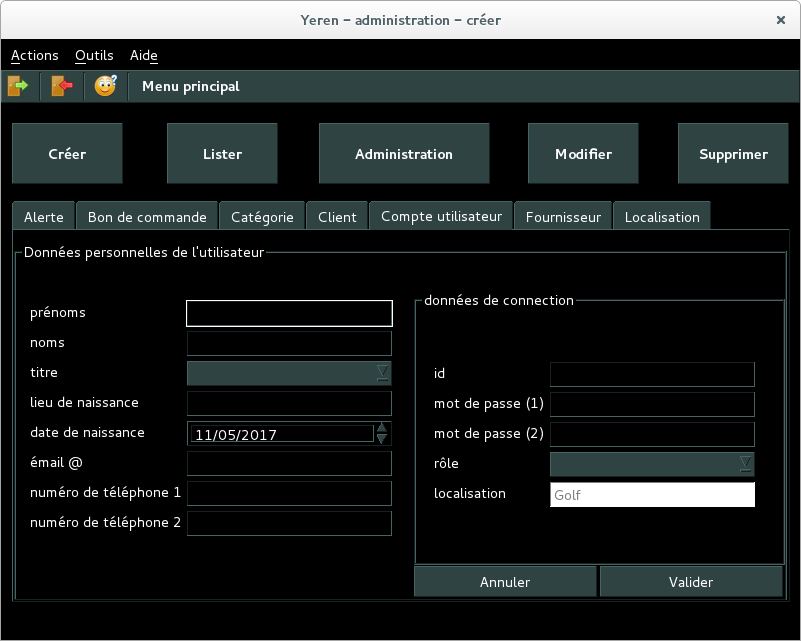
\includegraphics[scale=0.45]{images/compte-utilisateur-creer.png}
	\caption{L'interface graphique pour cr\'eer un compte utilisateur.}
	\label{fig:admin-comptes-utilisateurs-creer}
\end{figure}

La figure~\ref{fig:admin-comptes-utilisateurs-creer} illustre
l'interface graphique de \yeren pour cr\'eer un nouveau
compte utilisateur.

\procparagraph{Proc\'edure pour cr\'eer un compte utilisateur}
\begin{enumerate}[1)]
	\item \`A partir de l'interface graphique de l'acceuil de
		l'administration (voir figure~\ref{fig:fenetre-administrateur}),
		on clique sur l'onglet intitul\'e \textbf{op\'erations}. 
		
	\item Choisir '\textbf{cr\'eer}' dans le '\emph{combo box
		op\'erations}'.
		
	\item Choisir '\textbf{un compte utilisateur}' dans
		le '\emph{combo box objets}'. Vous \^etes automatiquement
		conduit \`a la fen\^etre illustr\'ee par la
		figure~\ref{fig:admin-comptes-utilisateurs-creer}.
		
	\item Saisissez les informations requises dans les champs
		de texte suivants:
		\begin{enumerate}[1)]
			\item pr\'enoms
			\item noms
			\item titre			
			\item lieu de naissance \optionel
			\item date de naissance \optionel
			\item \'email \optionel
			\item num\'ero de t\'el\'ephone 1 \optionel
			\item num\'ero de t\'el\'ephone 2 \optionel
			\item num\'ero de contribuable \optionel
			\item id
			\item mot de passe (1)
			\item mot de passe (2)			
			\item r\^ole.
		\end{enumerate}
		
	\item Cliquer sur le bouton \bouton{Valider} pour
		valider votre travail.	
\end{enumerate}


%%%%%%%%%%%%%%%%%%%%%%%%%%%%%%%%%%%%%%%%%%%%%%%%%%%%%%%%%%%%%%%%%%%%%%%%%%%%%%%%%

\newpage
\nxsubsection{Lister les comptes utilisateurs}
\index{lister les comptes utilisateur}

\begin{figure}[!htpb]
	\centering
	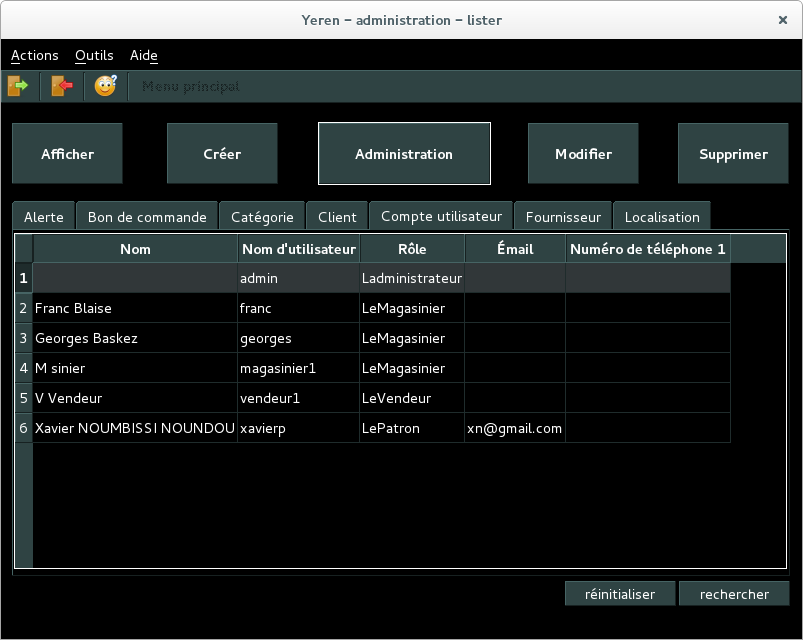
\includegraphics[scale=0.45]{images/compte-utilisateur-lister.png}
	\caption{L'interface graphique pour lister les comptes utilisateurs.}
	\label{fig:admin-comptes-utilisateurs-lister}
\end{figure}

La figure~\ref{fig:admin-comptes-utilisateurs-lister}
illustre l'interface graphique de \yeren qui liste les
comptes utilisateurs.

\procparagraph{Proc\'edure pour lister les comptes utilisateurs}
\begin{enumerate}[1)]
	\item \`A partir de l'interface graphique de l'acceuil de
		l'administration (voir figure~\ref{fig:fenetre-administrateur}),
		on clique sur l'onglet intitul\'e \textbf{op\'erations}. 
		
	\item Choisir '\textbf{lister}' dans le '\emph{combo box
		op\'erations}'.
		
	\item Choisir '\textbf{un compte utilisateur}' dans
		le '\emph{combo box objets}'. Vous \^etes automatiquement
		conduit \`a la fen\^etre qui liste les comptes clients
		(figure~\ref{fig:admin-comptes-utilisateurs-lister}).
\end{enumerate}

%%%%%%%%%%%%%%%%%%%%%%%%%%%%%%%%%%%%%%%%%%%%%%%%%%%%%%%%%%%%%%%%%%%%%%%%%%%%%%%%%

\newpage
\nxsubsection{Modifier les d\'etails d'un compte utilisateur}
\index{modifier les d\'etails d'un compte utilisateur}

\begin{figure}[!htpb]
	\centering
	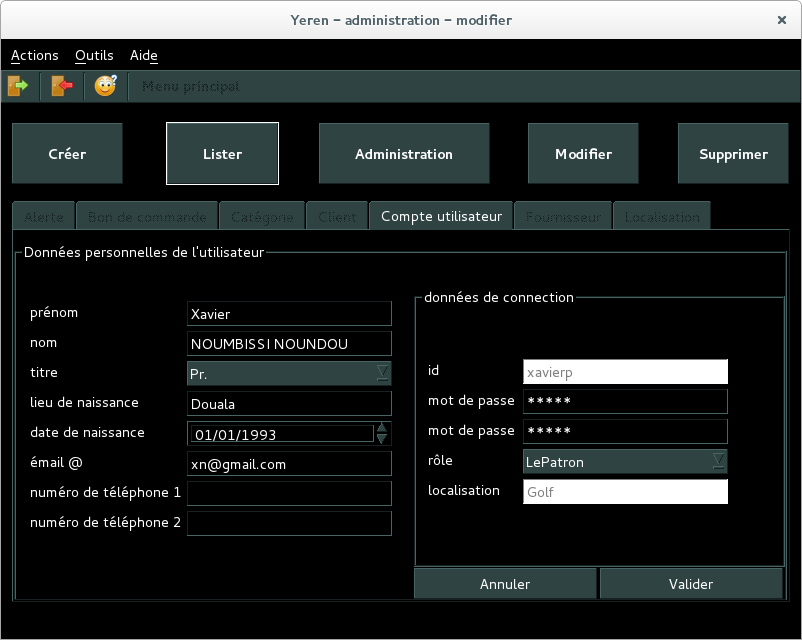
\includegraphics[scale=0.45]{images/compte-utilisateur-modifier.png}
	\caption{L'interface graphique pour modifier les d\'etails
			d'un compte utilisateur.}
	\label{fig:admin-comptes-utilisateurs-modifier}
\end{figure}

La figure~\ref{fig:admin-comptes-utilisateurs-modifier} illustre
l'interface graphique de \yeren pour modifier les d\'etails
d'un compte utilisateur.

\procparagraph{Proc\'edure pour modifier les d\'etails d'un compte utilisateur}
\begin{enumerate}[1)]
	\item \`A partir de l'interface graphique de l'acceuil de
		l'administration (voir figure~\ref{fig:fenetre-administrateur}),
		on clique sur l'onglet intitul\'e \textbf{op\'erations}. 
		
	\item Choisir '\textbf{lister}' dans le '\emph{combo box
		op\'erations}'.
		
	\item Choisir '\textbf{un compte utilisateur}' dans
		le '\emph{combo box objets}'. Vous \^etes automatiquement
		conduit \`a la fen\^etre illustr\'ee par la
		figure~\ref{fig:admin-comptes-utilisateurs-lister}.
		
	\item S\'electionner le compte utilisateur dont vous souhaitez
		modifier les d\'etails dans la liste des comptes
		utilisateurs affich\'ee.
		
	\item Cliquer sur le bouton \bouton{Modifier}. Les d\'etails
		du compte utilisateur sont affich\'es dans une nouvelle fen\^etre.
		
	\item Faites les modifications que vous souhaitez.
		
	\item Cliquer sur le bouton \bouton{valider} pour valider
		les modifications faites.
\end{enumerate}

%%%%%%%%%%%%%%%%%%%%%%%%%%%%%%%%%%%%%%%%%%%%%%%%%%%%%%%%%%%%%%%%%%%%%%%%%%%%%%%%%

\newpage
\nxsubsection{Supprimer un compte utilisateur}
\index{supprimer un compte utilisateur}

\begin{figure}[!htpb]
	\centering
	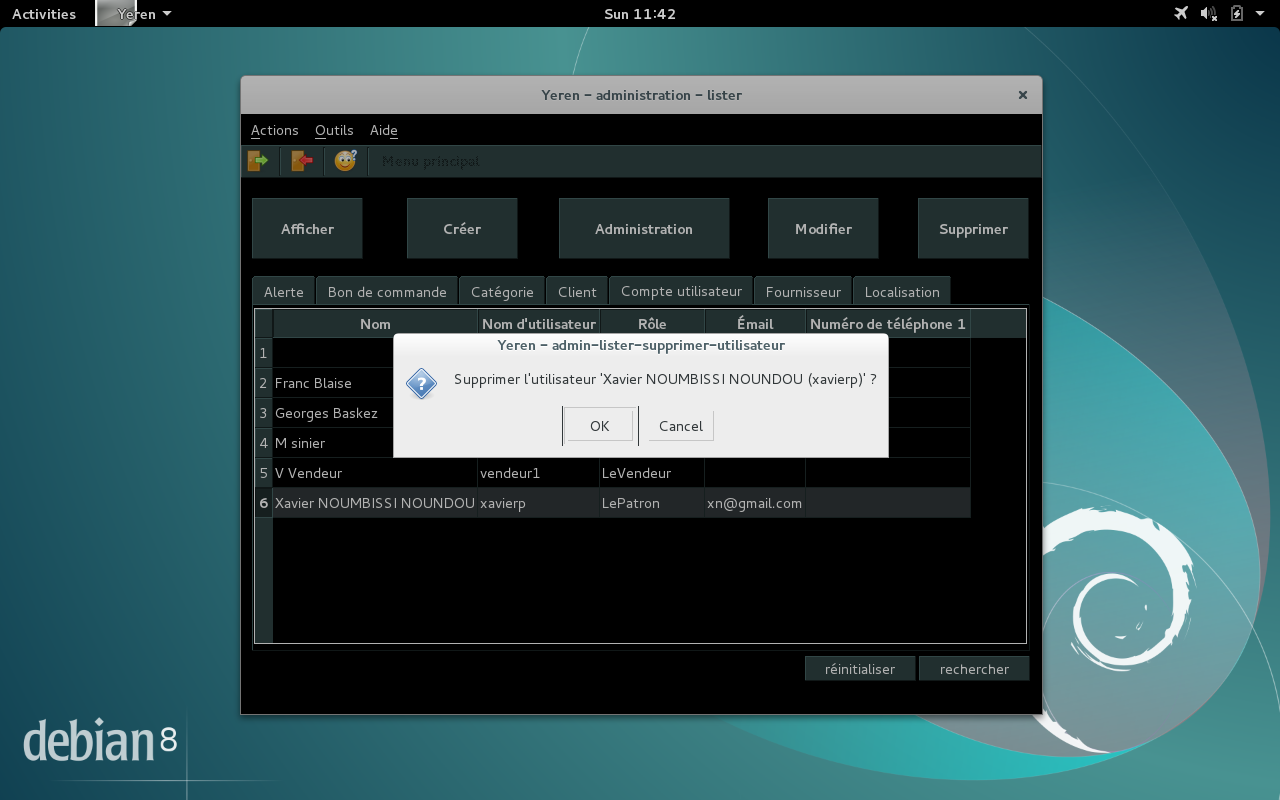
\includegraphics[scale=0.39]{images/compte-utilisateur-supprimer.png}
	\caption{L'interface graphique pour supprimer un compte utilisateur.}
	\label{fig:admin-comptes-utilisateurs-supprimer}
\end{figure}

La figure~\ref{fig:admin-comptes-utilisateurs-supprimer}
illustre l'interface graphique de \yeren pour supprimer
un compte utilisateur.

\procparagraph{Proc\'edure pour supprimer un compte utilisateur}
\begin{enumerate}[1)]
	\item \`A partir de l'interface graphique de l'acceuil de
		l'administration (voir figure~\ref{fig:fenetre-administrateur}),
		on clique sur l'onglet intitul\'e \textbf{op\'erations}. 
		
	\item Choisir '\textbf{supprimer}' dans le '\emph{combo box
		op\'erations}'.
		
	\item Choisir '\textbf{un compte utilisateur}' dans le
		'\emph{combo box objets}'. Vous \^etes automatiquement
		conduit \`a la fen\^etre illustr\'ee par la
		figure~\ref{fig:admin-comptes-utilisateurs-lister}.
		
	\item S\'electionner le compte utilisateur \`a supprimer
		dans la liste des comptes utilisateurs affich\'ee.
		
	\item Cliquer sur le bouton \bouton{Supprimer}. La question
		est ensuite pos\'ee si vous confirmer votre choix.
		Cliquer sur le \bouton{OK} pour confirmer votre choix.
\end{enumerate}
